

\section*{HS9. feladat:Gömb alakú főzőüst }
\addcontentsline{toc}{section}{HS/9. feladat}

\begin{tabular}{ | p{1.5cm} | p{11cm} | } 
	\hline
	Név: & Drávai Tamás László\\ 
	\hline
	Szak: & Mechatronikai mérnök \\ 
	\hline
	Félév: & 2019/2020 II. (tavaszi) félév \\ 
	\hline
\end{tabular}
\\
\\
\\HS9 feladat:\\
Határozzuk meg egy gömb alakú főzőüst falán keresztül előálló hőveszteséget (W).  Ha az üst belső átmérője 1.2 m az üst falának és szigetelő rétegének együttes vastagsága 100 mm. A belső felület hőmérséklete $T_1=140^0 C$, a külső felület hőmérséklete $T_2=50^0 C$, a hővezetési tényező $\lambda= 0.1396\frac{W}{mK}$.
\section*{ {Adatok:}}
$D_1=1.2 m \quad D_2=1.4 m \quad \lambda=0.1396  \dfrac{W}{mK} \quad \delta=0.1m$ falvastagság \\


\section*{Feladat megoldás}
$
\dot{Q} =\pi\cdot \lambda\cdot\bigtriangleup T \dfrac{D_1 \cdot D_2}{\delta}
\\
\\
\dot{Q}=\pi \cdot 0.1396 \dfrac{W}{mK} \cdot  90K \cdot\dfrac{1.2m \cdot 1.4 m}{0.1m}\\
\\
\dot{Q}=663.11 W $\\
\\
\\
A fözőüst falán keresztül fellépő hőveszteség az 663.11 W.\\
%%%%%%%%%%%%%%%%%%%%%%%%%%%%%%%%%%%%%%%%

\begin{figure}[h]
	\centering
	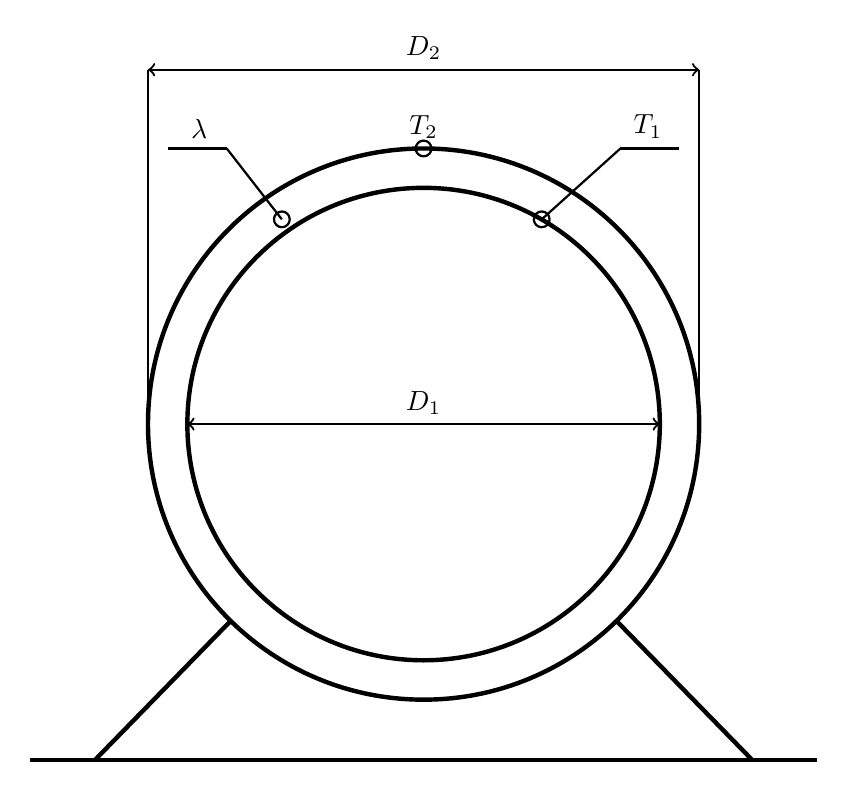
\begin{tikzpicture}
	%\draw[] (-6, -6) rectangle (6, 6); rajz keret
	\draw[color =black, ultra thick] (0, 0) circle (30 mm); %belső fal
	\draw[color =black,ultra thick] (0, 0) circle (3.5 ) ;%külső fal
	\draw[thick,<->] (-3,0) -- (3,0);% méretnyíl
	\draw (0,0)  node[above] {$ D_1  $};
	\draw[thick,<->] (-3.5,4.5) -- (3.5,4.5); %felső méretnyíl
	\draw (0,4.5)  node[above] {$ D_2  $};
	\draw [thick] (-3.5,0) -- (-3.5,4.5) (3.5,0) -- (3.5,4.5); %%felső méretnyíl oldalt
	\draw [ultra thick] (-2.45,-2.5) -- (-4.175,-4.2675) (2.45,-2.5) -- (4.175,-4.2675); %lábak
	\draw [ultra thick] (-5,-4.2675) -- (5,-4.2675) ;%földvonal
	%földvonalak
	fill[pattern={Lines[angle=45, distance=2mm]}] (-5, 0) rectangle (5, -0.5);
	%T1
	\draw [thick] (1.5,2.6) circle (0.1) (1.5,2.6) -- (2.5,3.5)  ;
	\draw [thick]  (2.5,3.5) -- (3.25,3.5) ;
	\draw [thick](2.85,3.5)  node[above] {$T_1$};
	% lambda
	\draw [thick] (-1.8,2.6) circle (-0.1) (-1.8,2.6) -- (-2.5,3.5)  ;
	\draw [thick]  (-2.5,3.5) -- (-3.25,3.5) ;
	\draw (-2.85,3.5)  node[above] {$\lambda$};
	%T2
	\draw [thick] (0,3.5) circle (0.1) ;
	\draw (0,3.5)  node[above] {$T_2$};
	
	\end{tikzpicture}
	\caption{Gömb alakú főzőüst }
\end{figure}

\begin{figure}
	%\centering
	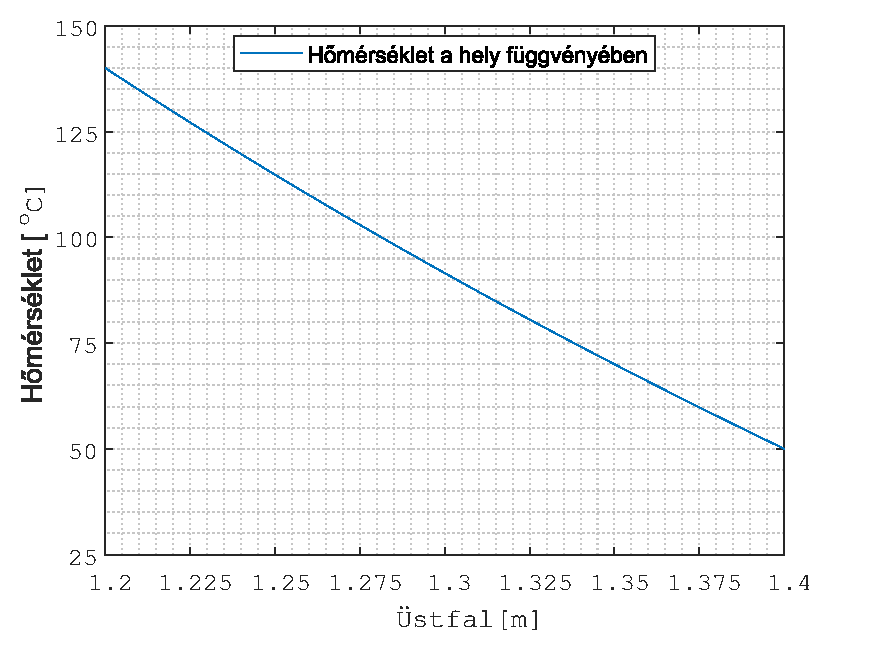
\includegraphics[width=1\linewidth]{homersekletfuggvenyHS9.eps}
	\caption{}
	\label{fig:waveforms}
\end{figure}
